\subsection{Lab13: Transmisor FM Estereo FIFO}

%*********************
\begin{frame}{}

\pgfdeclareimage[width=\paperwidth,height=\paperheight]{bg}{imagenes/fondo_lab}
\setbeamertemplate{background}{\pgfuseimage{bg}}

\bfseries{\textrm{\LARGE Lab13\\ \Large Transmisor FM Estereo FIFO}}
\raggedright
\end{frame}
%*********************

\begin{frame}{Introducción}

\pgfdeclareimage[width=\paperwidth,height=\paperheight]{bg}{imagenes/fondo3}
\setbeamertemplate{background}{\pgfuseimage{bg}}

Se realizará la retransmisión de una emisora online utilizando el transmisor de FM estéreo construido previamente en GNU radio (practica anterior); se aprovechará  la característica de un archivo “conducto” o “tubería” el cual nos permite que procesos separados se comuniquen sin haber sido diseñados para funcionar juntos; gracias a la herramienta mpg123 es posible alimentar un archivo FIFO que se comporta como tubería; es decir en la medida que ingresan los bits de información de la emisora online en la “tubería”, así mismo son extraídos por el transmisor de radio FM estéreo.

\end{frame}
%---------------------------------

\begin{frame}{Esquema general}
    
\begin{figure}[H]
\centering
\vspace{-3mm}
\includegraphics[width=\textwidth]{parte3/lab13/pdf/lab13_1.pdf}
\end{figure}
    
\end{frame}
%---------------------------------

\begin{frame}{Obtención URL emisora online}
    
\begin{figure}[H]
\centering
\vspace{-3mm}
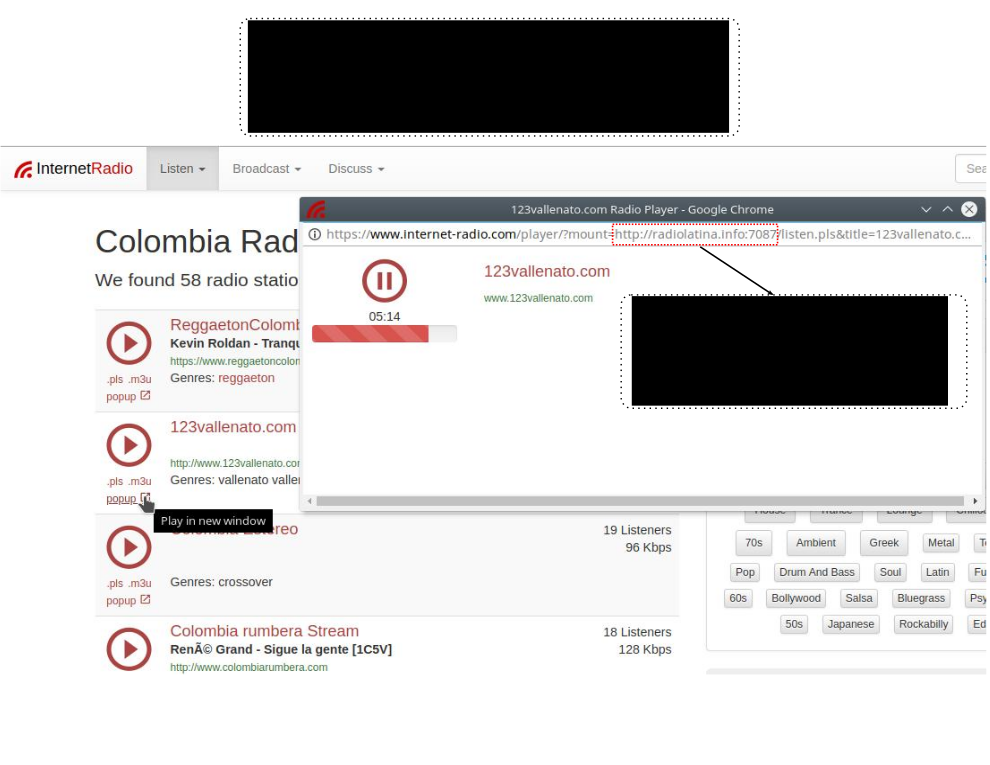
\includegraphics[width=.9\textwidth]{parte3/lab13/pdf/lab13_2.pdf}
\end{figure}
    
\end{frame}
%---------------------------------

\begin{frame}{Creación archivo FIFO}

Existe un tipo de tubería que puede ser descrita como una tubería "con nombre", también denominada FIFO que sus siglas traducen "Primero en entrar, primero en salir" y se refiere a la propiedad de que el orden de bytes entrante es el mismo que sale.

\begin{itemize}
    \item {Mediante el uso de consola procedemos a introducir el comando mkfifo, que nos permite crear el archivo FIFO.
    
    \begin{block}{}
    \texttt{
    \ \ \ mkfifo emisora\_online.fifo}
    \end{block}
    }
    \item {Mediante la herramienta mpg123 se procede a alimentar el archivo FIFO con una emisora online.
    
    \begin{block}{}
    \texttt{
    \ \ \ mpg123 -r44100 --stereo -s http://radiolatina.info:7087>emisora\_online.fifo}
    \end{block}
    }
\end{itemize}
\end{frame}
%---------------------------------

\begin{frame}{Creación archivo FIFO}

La opción "--stereo" permite realizar una transmisión de tipo estéreo, utilice “-m” para realizar una transmisión de tipo monofónica.\vspace{2mm}

Con la ayuda de la apción “-r” podemos definir la tasa de muestreo, por ejemplo "-r44100" convierte la frecuencia de muestreo a 44100 muestras por segundo. \vspace{2mm}

Es importante el uso del comando “-s” que nos permite que las muestras de audio decodificadas se escriben en la salida estándar es decir en consola, en lugar de reproducirlas a través del dispositivo de audio; gracias a esta característica se puede llevar a cabo el concepto del uso de tuberías que suelen ser alimentadas a través de pantalla.

\end{frame}
%---------------------------------

\begin{frame}{Creación archivo FIFO}

\begin{itemize}
    \item {Si se desea realizar una prueba previa a la transmisión, es posible escuchar la emisora de igual manera mediante la herramienta mpg123; recuerde eliminar el comando “-s” para que las muestras de audio no se muestren en pantalla y sean reproducidas a través del dispositivo de audio.
    
    \begin{block}{}
    \texttt{
    \ \ \ mpg123 -r44100 --stereo  http://radiolatina.info:7087}
    \end{block}
    }
\end{itemize}
\end{frame}
%---------------------------------

\begin{frame}{Explicación bloques extras}

\begin{figure}[H]
\centering
\vspace{-3mm}
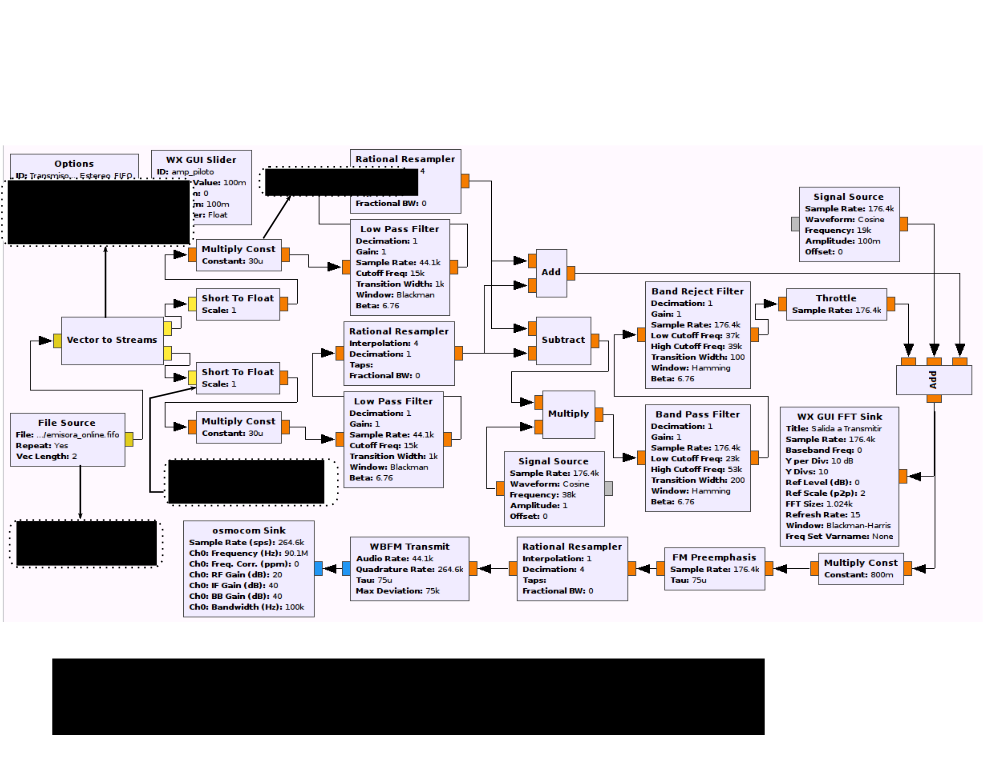
\includegraphics[width=\textwidth]{parte3/lab13/pdf/lab13_3.pdf}
\end{figure}
\end{frame}
%---------------------------------

\begin{frame}{Espectro de señal a transmitir}

\begin{figure}[H]
\centering
\vspace{-3mm}
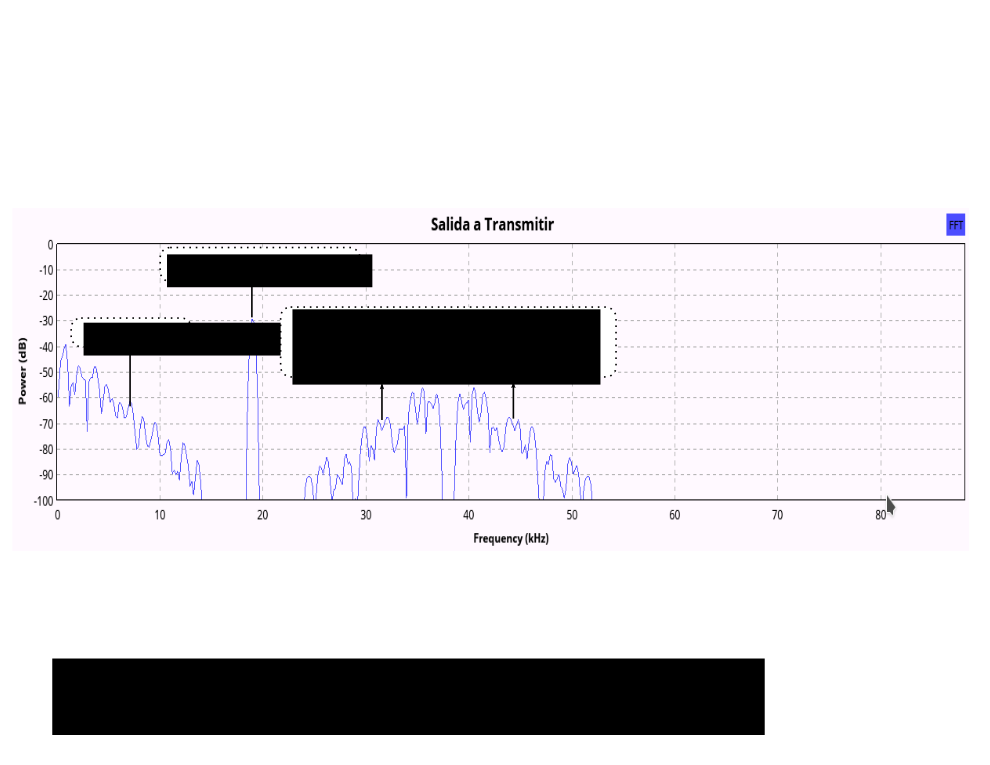
\includegraphics[width=\textwidth]{parte3/lab13/pdf/lab13_4.pdf}
\end{figure}
\end{frame}
%---------------------------------